\section{Desarrollo}
  
\subsection{General}

\subsubsection{Vertical Mirror}

Copia la primera parte de la imagen en la segunda parte, espej\'andola con respecto a la vertical. Cada pixel se transporta entero de acuerdo a la distancia que tiene a la l\'inea central de la imagen. Para cada pixel $p$ se eval\'ua lo siguiente:\\
\begin{center}
$Posicion(p') = ancho - Posicion (p)$
\end{center}
\subsubsection*{Pseudo-C\'odigo}
\begin{verbatim}
para cada fila de 0 a altura-1
     para cada pixel de 0 a ancho/2 sobre esta fila
          copiar el pixel de pos_P en: ancho - pos_P
\end{verbatim}
\subsubsection*{Ejemplo}
\begin{center}
  \begin{figure}[H]
  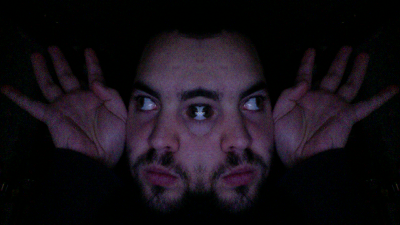
\includegraphics[scale=0.60]{imgs/vmirr.png}
  \end{figure}  
\end{center}

\subsubsection{Negative}

Este filtro invierte los colores en cada pixel de la imagen. Para invertir un pixel se realiza la diferencia con 255 de cada canal.\footnote{http://es.wikipedia.org/wiki/Inversion\_(imagen)}
Dado un pixel $p$:\\

\begin{center}

Neg(R) = 255 - R

Neg(G) = 255 - G

Neg(B) = 255 - B
 
\end{center}
\subsubsection*{Pseudo-C\'odigo}
\begin{verbatim}
para cada fila de 0 a altura-1
     para cada pixel de 0 a ancho sobre esta fila
          en la pos_P del pixel_P calcular: - pixel_P
\end{verbatim}
\subsubsection*{Ejemplo}
\begin{center}
  \begin{figure}[H]
  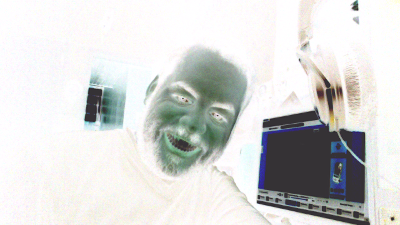
\includegraphics[scale=0.60]{imgs/neg.png}
 % \caption{}
  \end{figure}  
\end{center}

\subsubsection{Stretch (zoom x2)}

Transforma la imagen de forma tal que cada pixel $p$ se copia 3 veces en las posiciones de sus vecinos a izquierda, abajo y diagonal, generando una imagen resultado que es equivalente a hacer zoom sobre el primer cuadrante de la imagen original.\footnote{http://en.wikipedia.org/wiki/Nearest-neighbor\_interpolation}
\subsubsection*{Pseudo-C\'odigo}
\begin{verbatim}
para cada fila de 0 a altura/2
     para cada pixel de 0 a ancho/2 sobre esta fila
          en la pos_P del pixel_P copiar pixel_P
          copiar pixel_P a la derecha, abajo y diagonal
\end{verbatim}
\subsubsection*{Ejemplo}
\begin{center}
  \begin{figure}[H]
  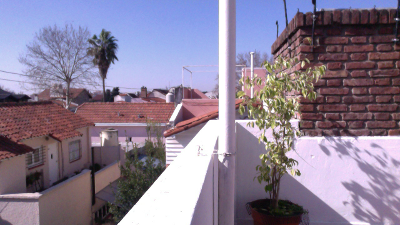
\includegraphics[scale=0.60]{imgs/stretch1.png}
  \end{figure}  
  \begin{figure}[H]
  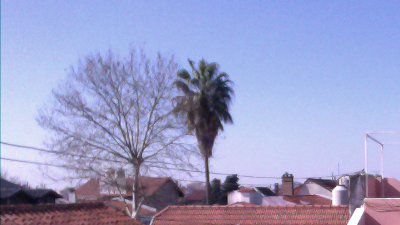
\includegraphics[scale=0.60]{imgs/stretch2.png}
  \end{figure}  
\end{center}  

\subsubsection{Edge (Sobel + colores)}

Este filtro detecta los bordes utilizando el algoritmo Sobel. Se examina cada pixel de la imagen, para cada uno se multiplica el valor de este pixel y los valores de los 8 circundantes por el valor correspondiente de la matriz. El pixel del centro de la matriz regula su valor de acuerdo al valor resultante de la operaci\'on. La dificultad est\'a puesta en aprovechar las bondades de las instrucciones SIMD y sus capacidades para trabajar en grandes lotes.\footnote{$http://en.wikipedia.org/wiki/Sobel_operator)$} \\
La matriz de convolucion X es:
\begin{center}
$\begin{bmatrix}
  +1 & 0 & -1 \\
  +2 & 0 & -2 \\
  +1 & 0 & -1
 \end{bmatrix}$
 \end{center}
La matriz de convolucion Y es:
\\
\begin{center}
$\begin{bmatrix}
  +1 & +2 & +1 \\
  0 & 0 & 0 \\
  -1 & -2 & -1
 \end{bmatrix}
$\end{center}

\subsubsection*{Pseudo-C\'odigo}
\begin{verbatim}

se hace una pasada para calcular las derivadas parciales en X
se hace otra pasada para calcular las derivadas parciales en Y
    se genera el gradiente de (X,Y) y se guarda en cada pixel
\end{verbatim}
\subsubsection*{Ejemplo}
\begin{center}
  \begin{figure}[H]
  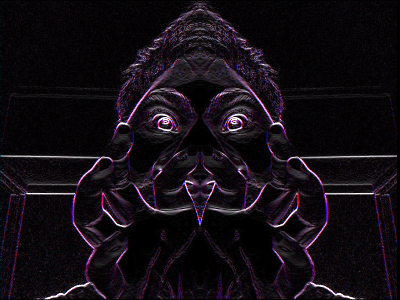
\includegraphics[scale=0.60]{imgs/sobel.png}
  \end{figure}  
\end{center}  

\subsubsection{Bona (distancia a un color)}

El algoritmo genera un filtro y una conversi\'on en la imagen. Son utilizados dos par\'ametros de entrada: color y tamaño de la ventana. Por cuestiones est\'eticas se decidi\'o utilizar el rojo como color par\'ametro y la medida de la ventana se acomoda de acuerdo al nivel de apertura del obturador e ISO de la c\'amara. En muchas webcams estos par\'ametros son manejados por el driver mismo, quedando el threshold como \'unico par\'ametro para obtener el efecto deseado.

Respecto de la l\'ogica de la rutina, se mide la distancia geom\'etrica de cada pixel al color par\'ametro y, en caso de ser cercano, se deja como se encontraba. En caso de tener una distancia mayor a la sugerida por el tamaño de ventana, se monocromatiza el pixel. El efecto deseado destaca en la imagen el color par\'ametro elegido.\footnote{http://stackoverflow.com/questions/9018016/how-to-compare-two-colors}

\subsubsection*{Pseudo-C\'odigo}
\begin{verbatim}
para cada pixel p de la imagen:
    si la distancia de colores entre p y rojo es mayor a la ventana
        se monocromatiza el pixel con el algoritmo (R+2G+B)/4
\end{verbatim}
\subsubsection*{Ejemplo}
\begin{center}
  \begin{figure}[H]
  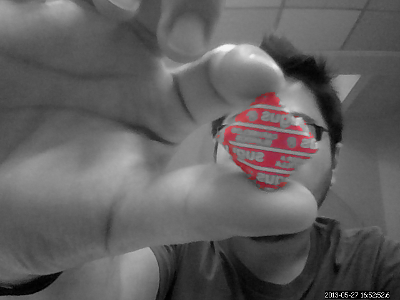
\includegraphics[scale=0.60]{imgs/bona.png}
  \end{figure}  
\end{center}  

\subsubsection{Pixelate}

Como su nombre lo indica, el algoritmo pixela la imagen mediante la p\'erdida de informaci\'on de la misma. Para ello, construye una matriz cuadrada de tamaño param\'etrico y replica la informaci\'on del pixel (0;0) en el resto de los p\'ixeles de la matriz. La imagen resultante simula haber perdido calidad y se asemeja a la de los viejos personajes de los juegos de 8 bits. La complejidad del algoritmo est\'a ubicada en hacerlo param\'etrico al tamaño de la matriz y que, a pesar de que el tamaño sea variable, se siguieran utilizando las bondades del procesamiento en paralelo que proveen las instrucciones SIMD.\footnote{http://en.wikipedia.org/wiki/Pixelation}

\subsubsection*{Pseudo-C\'odigo}
\begin{verbatim}
para cada sub-matriz de n x n pixels
    se toma el valor de (0,0) y se lo copia en el resto de las posiciones de la sub-matriz
\end{verbatim}

\subsubsection*{Ejemplo}
\begin{center}
  \begin{figure}[H]
  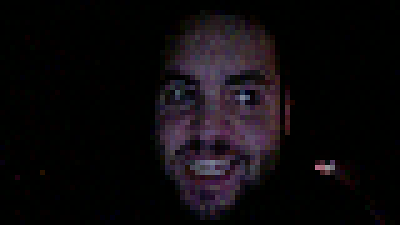
\includegraphics[scale=0.60]{imgs/pix.png}
 % \caption{}
  \end{figure}  
\end{center}

\subsubsection{Instagram}

El efecto que propone el filtro es la simulaci\'on de que la imagen fue tomada por una camara antigua. El objetivo es darle un aspecto tostado al video. Este mismo efecto fue popularizo por la red social Instagram y es la acumulaci\'on de otros efectos sobre la misma imagen. Para lograrlo se le baja el brillo, se le sube el contraste y se ruboriza la imagen. La ruborizaci\'on de la imagen la resolvimos ubicando a los p\'ixeles en dos grupos seg\'un su distancia al color negro (\#0,0,0), los que mas distancia ten\'ian eran ruborizados con menos fuerza (10h) y los dem\'as con 16h para obtener el efecto final tostado y que no se rompiera la continuidad con la diferencia de color.\footnote{http://net.tutsplus.com/tutorials/php/create-instagram-filters-with-php/}

\subsubsection*{Pseudo-C\'odigo}
\begin{verbatim}
Para cada pixel de la imagen:
    si dista del negro mas que la ventana
        se le suman 10h a la componente R
    si la distancia no es suficiente
        se le suman 16h a la componente R
Luego, para cada pixel de la imagen:
    se reduce el brillo, restando 40 a todas las componentes R, G y B
    se aumenta el contraste un 25%
\end{verbatim}

\subsubsection*{Ejemplo}
\begin{center}
  \begin{figure}[H]
  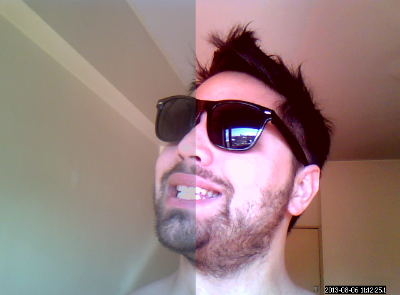
\includegraphics[scale=0.60]{imgs/insta.png}
 % \caption{}
  \end{figure}  
\end{center}

\subsubsection{Monochrome}

Pasa la imagen a escala de grises.\footnote{http://www.tannerhelland.com/3643/grayscale-image-algorithm-vb6/} Para monocromatizar cada pixel $p$, se considera la cuenta:
\begin{center}
$ (R + 2G + B ) * 1/4 $
\end{center}
\subsubsection*{Pseudo-C\'odigo}
\begin{verbatim}
para cada pixel p en la imagen:
     el valor de R, G y B se pisa con el resultado de la cuenta: (R + 2G + B ) * 1/4
\end{verbatim}

\subsubsection*{Ejemplo}
\begin{center}
  \begin{figure}[H]
  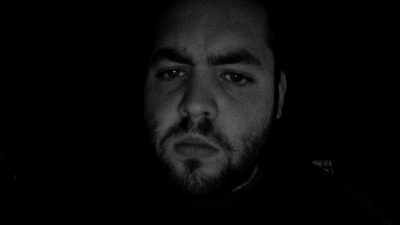
\includegraphics[scale=0.60]{imgs/mono.png}
  \end{figure}  
\end{center}  

\subsubsection{Channel}

Este filtro considera un \'unico canal (el R, G o B) y filtra los otros dos. La imagen resultante es monocrom\'atica roja-negro, verde-negro o azul-negro.
\subsubsection*{Pseudo-C\'odigo(Red)}
\begin{verbatim}
para cada pixel p en la imagen:
    el valor de G y B se pisa con 0   
\end{verbatim}

\subsubsection*{Ejemplo}
\begin{center}
  \begin{figure}[H]
  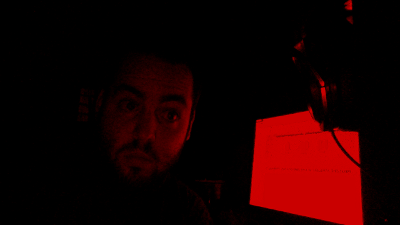
\includegraphics[scale=0.60]{imgs/chan.png}
  \end{figure}  
\end{center}  

\subsubsection{Median}

Dado un pixel $p$, el filtro calcula el promedio de cada vecindad. Las vecindades son de 5x5 pixels y el efecto resultante produce una disminuci\'on del ruido en la imagen. Como efectos colaterales, se pierde un poco de brillo y detalle en la imagen.\footnote{$http://en.wikipedia.org/wiki/Median_filter$}
\subsubsection*{Pseudo-C\'odigo}
\begin{verbatim}
para cada fila entre 2 y altura - 2:
    para cada columna entre 2 y ancho - 2:
        para cada pixel p:
            se calcula el promedio R, G y B de todos los 8 vecinos
            se pisa p con el promedio R, G y B de la vecindad
\end{verbatim}

\subsubsection*{Ejemplo}
\begin{center}
  \begin{figure}[H]
  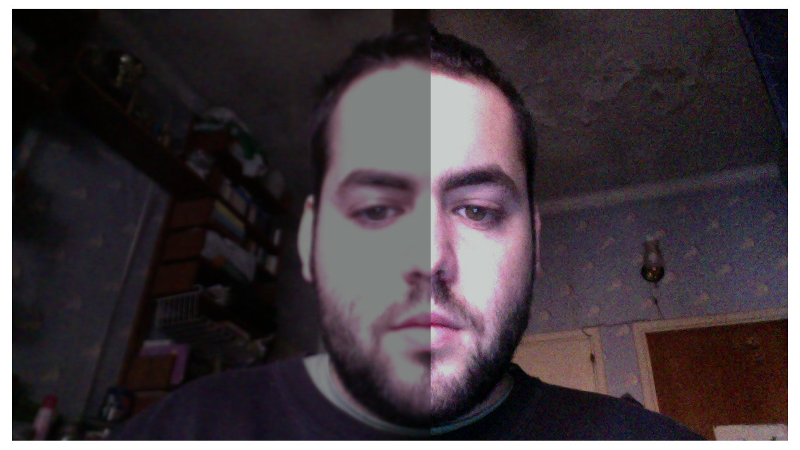
\includegraphics[scale=0.40]{imgs/median.png}
  \end{figure}  
\end{center}  
